\documentclass[12pt]{article}
\usepackage[utf8]{inputenc}
\usepackage{natbib}
\usepackage[frenchb]{babel}
\usepackage{listings}
\usepackage{babel}
\author{'Sue Enzo'}
\author{'Rebut Armand'}
\usepackage{amsmath}
\usepackage{graphicx}
\usepackage[T1]{fontenc}
\usepackage{hyperref}
\usepackage{fancyhdr}
\usepackage{lastpage}
\usepackage{graphicx, wrapfig, subcaption, setspace, booktabs}
\usepackage{fourier}
\usepackage[protrusion=true, expansion=true]{microtype}
\usepackage{hyperref}
\usepackage[margin=2.5cm]{geometry}
\renewcommand{\baselinestretch}{1.3}
\usepackage{color}
\begin{document}
\begin{titlepage}
	\parindent0pt
	\fbox{%
		\begin{minipage}{\dimexpr\linewidth-2\fboxsep-2\fboxrule}
			\centering\Large\bfseries
			\vskip1cm
			Université de Caen\par
			Master Informatique\par
			Année universitaire 2019/2020\par
			Rapport Technique
			\vskip0.5cm \kern0pt
		\end{minipage}%
	}%
	\vskip0pt plus 0.1fil
	\fbox{%
		\begin{minipage}{\dimexpr\linewidth-2\fboxsep-2\fboxrule}
			\centering\Large\bfseries
			\vskip1cm
			Projet tutoré:\par
			Implémentation d'un système de réalité augmentée orienté image avec interaction multi-utilisateurs
			
			\vskip1cm \kern0pt
		\end{minipage}%
	}%
	\vskip0.5cm
	\textbf{\large{Enzo SUE \hfill 21606200\newline Armand REBUT\hfill 21607828}}
	\newline
	\textbf\large\center\Large
	Enseignant référent: Loïs Vanhée

	\begin{center}		
\includegraphics[width=0.35\textwidth]{logounicaen.png}
	\end{center}
	\leavevmode
	\begin{minipage}{\dimexpr\linewidth/2-.4pt-.25cm\relax}
	\end{minipage}%
	\hskip.25cm \vrule width.8pt \hskip.25cm
	\begin{minipage}{\dimexpr\linewidth/2-.4pt-.25cm\relax}
	\end{minipage}%
	\small
Ce projet s'intègre dans l'initiative "la confrérie du code", initiée par Loïs Vanhée. Cette initiative vise à permettre aux apprenants de développer, en plus des compétences techniques classiques, la panoplie des compétences impliquées par la mise en place de projets en pratique (communication, organisation, collaboration, etc) et de garder une vision réflective sur leur propre développement. Le rapports pédagogique décrivent l'évolution de notre développement durant tout le projet.
\end{titlepage}



\newpage
\tableofcontents
\newpage









\section{Remerciement}

Nous aimerions présenter nos remerciements à notre enseignant référent Mr Loïs VANHEE.
Nous voudrions également lui témoigner notre gratitude pour son soutien et le
temps qu'il nous a accordé afin de mener notre travail à bon port. 
\newpage

\section{Introduction}
Ce projet de réalité augmenté à capter notre attention pour plusieurs raisons : 
\begin{itemize}
    \item Il s'agit d'une technologie qui nous était inconnu, nous avions envie de la découvrir.
    \item Le sujet était extrêmement libre, nous avions une grande liberté durant tout le projet
\end{itemize}

\medbreak
\textit{La réalité augmentée} est aujourd'hui utilisé dans plus en plus de domaine, que ce soit l'éducation, la médecine ou pour des applications plus ludiques. Ce développement suit la progression des technologies permettant de l'utiliser, \textit{presque tout les portables aujourd'hui} disposent d'une puissance suffisante pour le faire marcher. Bien que possédants certains problèmes tels que ce soit la difficulté pour les applications mobiles de trouver des points pour créer l'espace ou les problèmes au niveau de la vie privée, cela ne réduit pas l'engouement vers cette technologie. L'une des principale raison de cet essor est sa flexibilité, \textit{beaucoup d'entreprises utilisent aujourd'hui cette technologie } pour mettre en valeur leurs produits ou permettre à l'acheteur de visualiser ce même produit dans un endroit tel que chez lui.
\medbreak
Beaucoup d'applications de ce type sont aujourd'hui mono-utilisateur car utilisées pour donner des informations à un simple utilisateur. Sa plus grande part d'utilisation sont les applications de type visualisation d'un produit dans un environnement. Il s'agit simplement d'une projection de l'objet dans la réalité reproduite avec la caméra de sa tablette ou son téléphone

\medbreak

Ce projet s'inscrit dans le cadre de notre formation de Master informatique à l'Université de Caen Normandie. Dans ce projet, nous nous sommes fixés comme objectif de \textit{réaliser une application utilisant la réalité augmentée et  étant multi-utilisateur}. Nous voulons que ce projet sois \textit{déployable sur Android}, quel soit ludique, que chaque personne puisse apporter sa pierre à l'édifice objectif.
\medbreak
Pour valider ce projet, nous avons choisis de créer \textit{une application de dessin en réalité augmentée} où chaque personne pouvait dessiner avec les autres afin de réaliser une forme plus ou moins complexe et être noté sur celle-ci. Nous l'avons ensuite déployer sur plusieurs smartphones, nous pouvons suivre ce qu'il se passe via une base de données mise à jour en temps réel et via les écrans des smartphones participant à l'expérience où qu'ils soient.
Cette application a une portée plus grande que juste ce dessin car suite à la coopération avec les membres d'un autre groupe travaillant sur la réalité augmentée au niveau localisation, l'aboutissement final du projet sera \textit{un jeu en équipe dans une grande zone} (exemple: la ville de Caen,...), chaque équipe possédera plusieurs points à attaquer. Pour attaquer un point, chaque équipe devra réaliser un dessin plus ou moins complexe au lieu où se trouve le point en 3D. L'équipe possédant tout les points gagnerait la partie.
\medbreak
Ce projets impliqués plusieurs difficultés techniques: Chaque personne doit pouvoir jouer avec les autres peut-importe son emplacement. Le dessin en 3 dimension était une nouvelle technologie tout comme le langage et la mise en place d'un jeu en temps réel. 
\medbreak
Ce rapport vous présentera d'abord l'état de l'art, les logiciels et technologies existant déjà en rapport à la réalité augmentée. Suite à ça nous feront une comparaison des outils existant et expliquerons ce que nous avons choisis et pourquoi les avoir choisis. Enfin, nous allons parler de la création et l'implémentation des objectifs dans l'application.

\medbreak
Nous pouvons voir sur les photos ci-dessous l’utilisation de l’application. La première photo montre la réalisation d’un premier dessin par le premier utilisateur et la vue de ce dessin par le joueur 2 dans la photo suivante. Le joueur 2 a ensuite compléter le dessin. Dans la dernière photo, le joueur 1 à vérifier avec le modèle. 

\begin{center}		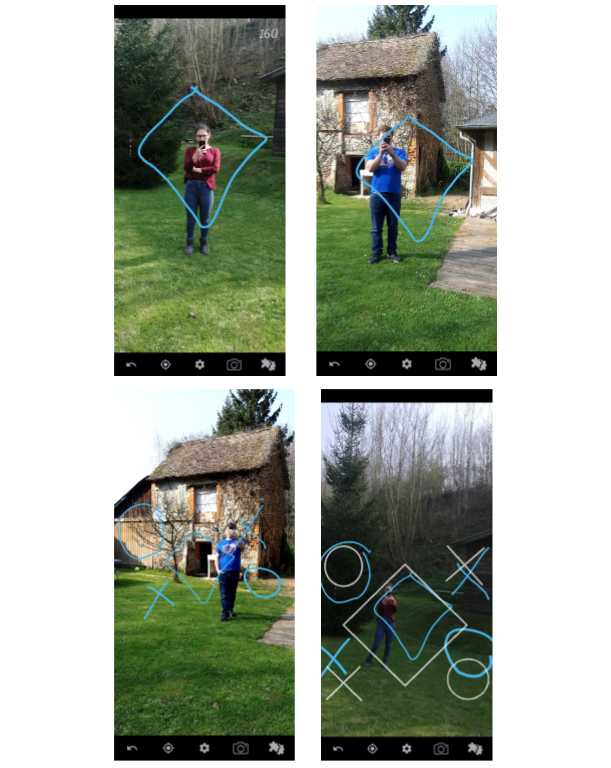
\includegraphics[width=0.7\textwidth]{intro.png}
\end{center}



\section{Objectifs}
Les objectifs de ce projet est de :
\begin{itemize}
\item réaliser une application concrète à l'aide du code de l'année précédente, c'est à dire une application utilisant la réalité augmentée et permettant des interactions multi-utilisateurs avec cette les objets de cette nouvelle réalité
\item réaliser une journée de validation afin de valider notre projet
\end{itemize}


\section{Etat de l'art}
\subsection{La réalité augmentée}
Le principe de la réalité augmentée est de superposer des éléments virtuel au monde réel. Le tout en temps réel avec pour but de donner l'illusion de l'intégration de l'élément dans le monde qui l'entoure. Aujourd'hui assez répandue, notamment avec son accessibilité devenu trivial par l'avancement des smartphones actuel permettant l'utilisation de cette technologie.
Son fonctionnement est rendu possible par la détection de marqueur (dans une image ou un objet du monde réelle) qui permet le positionnement et le rajout des éléments virtuels. 
Cette technologie est utilisée dans de nombreux domaine comme le jeu vidéo, l'éducation, le bâtiment ou encore la navigation avec pour but,d'apporter des information sur l'environnement réel autour de l'utilisateur.


\subsection{Projet de l'année précédente}
L'année précédente, des étudiants ont réalisé une application de réalité augmentée.\par
Cette application utilisait une image possédant des marqueurs afin de reconnaitre l'environnement sur lequel la réalité augmentée devait avoir lieu. De là sortait un personnage avec lequel nous pouvions réaliser plusieurs actions plus ou moins simples à l'aide de boutons.
\newline
De plus, il possédait une interaction multi-utilisateur, en effet, 2 personnes scannant la carte pouvait accéder à la même salle depuis laquelle nous pouvions voir chaque personnage contrôlait par chaque joueur.
	\begin{center}		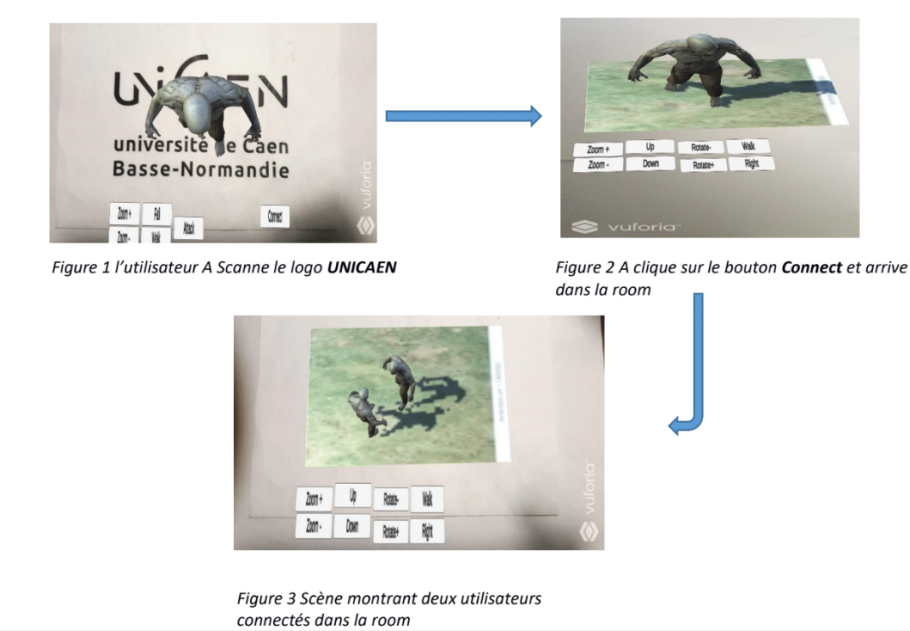
\includegraphics[width=0.9\textwidth]{projetAnneeDerniere.png}
	\end{center}
\par
Ce projet était très intéressant mais cependant, plusieurs attributs empêcher l'intégration de ce projet à l'intérieur du notre : tout d'abord, notre projet devait pouvoir se jouer sur des grandes zones sans préparation préalable excepté la création des équipes. Ainsi, il nous était impossible d'aller déposer des marqueurs sur toute la ville avant de lancer notre jeu. Nous devions donc repenser à comment réaliser la reconnaissance du terrain.


\section{Outils existant}
\par
Il existe plusieurs outils permettant de réaliser des applications de réalité augmentée. Nous avons commencé par nous intéresser à l'outil utilisé pour le projet de l'année dernière.
 Ce dernier est \textbf{Vuforia}, un plug in de Unity 3d qui fonctionne par reconnaissance de marqueur (photo Qr code), d'objet 3d et de forme. Ensuite, il y a \textbf{ARCore}, un framework de google
  reprenant sensiblement les fonctionnalité d'\textbf{ARkit} framework d'Apple. Ce dernier est capable de détecter l'environnement sans l'ajout de marqueur ou de préparation. Nous avons aussi
 pris connaissance donc de \textbf{ARKit} et \textbf{Easy AR} pour l choix de notre outil.

\subsection{Décision technique:}
\par
Nous avions, dans un premier temps, choisit d'utiliser Vuforia comme outil notamment pour sa simplicité et la possibilité de gérer les marqueur à distance. Mais au vu du choix de notre application, ARcore été un choix plus judicieux pour sa reconnaissance de l'environnement sans marqueur prédéfinis. Nous n'avons pas voulu utiliser ARkit car il est seulement disponible sur IOS or nous voulions développer un projet sur Android, bien plus répandu et installé sur les téléphones portables auxquels nous avions accès. Nous avons donc réalisé notre projet avec le Framework ARcore.

\par
Voici quelques critères que nous avons utilisé lors de notre recherche, organisé dans un tableau de comparaison:\newline
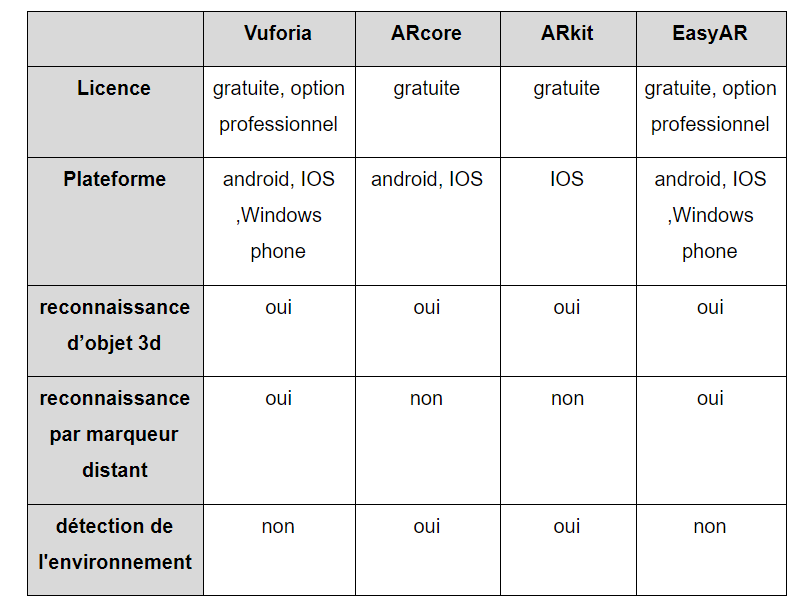
\includegraphics[width=0.9\textwidth]{tableauComparaison.png}

	
\section{Outils utilisés}
	\subsection{ARcore}
		\begin{itemize}
			\item Acquisition de l'image
		\end{itemize}
		\par
		ARcore étant un framework utilisé pour des applications Android, ce dernier demande l'autorisation et utilise la caméra de l'appareil pour la reconnaissance de l'environnement.

		\begin{itemize}
			\item Ajout d'objet virtuel
		\end{itemize}
		\par
		ARcore permet la visualisation d'objet 3d virtuellement , dans un environnement réel. ARcore peut prendre en compte les surface dans l'ajout de ces objets

		\begin{itemize}
			\item Détection de l'environnement
		\end{itemize}
		\par
		ARcore va être capable de reconnaître et se positionner dans un environnement réel. Pour cela ARcore va utiliser les capteur du téléphone comme l'accéléromètre pour détecter les mouvements ainsi que la caméra. Puis après une phase de calcul va créer des marqueurs pour se repérer.
		\par
		Mais cette fonctionnalité est à double tranchant , car cela réduit les appareils compatibles au vu de la puissance nécessaire.

		\begin{itemize}
			\item Reconnaissance des surfaces
		\end{itemize}
		\par
		Avec la détection de son environnement , ARcore et aussi capable de détecter les surfaces. Il peut ainsi repérer les surfaces horizontale et verticale. Cela permet de pouvoir placer des objets virtuels sur des tables , sols ou murs réels.
	\subsection{FireBase}
	\par
	FireBase est un service destiné au développement mobile et Web. Firebase est un outil regroupant plusieurs api et fonctionnalités intuitive facilitant de développement et la gestion. Le tout pouvant desservir une multitude d'utilisateurs en même temps. Dans ces multitudes de service nous pouvons trouver:
	\begin{itemize}
		\item Firebase authentification
	\end{itemize}
	\par
	Ce service permet de faciliter l'authentification des utilisateurs se connectant à nos application. Cela nous permet dans notre projet de disposer d'un système d'authentification sécurisée et facile à mettre en œuvre tout en pouvant profiter de l'authentification par compte Google,Twitter ou encore Facebook.
	\begin{itemize}
		\item Cloud Messaging
	\end{itemize}
	\par
	Permet la réception et l'envoie de notification . Il est possible d'envoyer des messages ou notifications aux utilisateurs de l'application via ce service.

	\begin{itemize}
		\item Realtime Database
	\end{itemize}
	\par
	Base de donnée NOSQL permettant le stockage et l'accès à l'information en temps réelle. Les utilisateurs peuvent recevoir et mettre à jour les données avec une synchronisation en temps réelle. Lorsque le terminal passe en mode hors ligne , Firebase utilise le cache pour pouvoir sauvegarder avant d'envoyer et mettre à jour les données lorsque l'appareil est de nouveau connecté .
\section{Réalisation technique}
\par
La réalisation du projet c'est déroulée en deux étape. Dans un premier temps nous avons pris en main le projet open source DrawAR afin de comprendre et réaliser notre application de dessin. Ensuite, nous avons intégrer la partie multi utilisateur.
	\subsection{Première partie}
	\par
	Pour commencer notre projet nous nous sommes donc concentrés sur la partie réalité augmentée. Et pour cela nous avons pris en main le Framework ARcore et fait des recherche sur des exemples de projets. Nous avons trouver un projet open source DrawAR (https://github.com/googlecreativelab/ar-drawing-java/blob/master/app/src/main/java/com/googlecreativelab/drawar/DrawAR.java)  Ce projet est une exxpérience de Google open-source afin de tester leur Framework. Nous nous sommes donc servi de ce projet comme base pour le notre, et avons décortiqué le programme pour le comprendre et se l'approprier. 
	\begin{itemize}
		\item Caméra
	\end{itemize}
	\par
	Pour un projet utilisant ARcore nous n'utilisons pas directement la caméra , nous faisons appel à l'objet Camera d'ARCore. Cette objet pourra permettre d'acquérir les information nécessaire pour la position de point dans l'espace.

	\begin{itemize}
		\item Vector3f
	\end{itemize}
	\par
	Les points sont représentés par des Vector3f. Ce vecteur et donc composé de 3 donnée : x, y et z. C'est grâce à ces points que le dessin sera réalisé.

	\begin{itemize}
		\item Les traits
	\end{itemize}
	\par
	Les différents traits qui seront réalisés seront donc constitués d'une multitude de point. Le dessin dans sa globalité sera sauvegarder dans une liste de liste de vecteur.

	\begin{itemize}
		\item LineShaderRenderer
	\end{itemize}
	\par
	LineShaderRenderer sera utilisé à chaque mouvement ou ajout de point. Cette classe permet de générer et afficher le dessin réaliser un l'ajoutant par dessus le flux de la caméra.
	\par
	Avant de commencer notre projet nous avons dû préciser dans le fichier build de notre application que nous voulions qu'il télécharge les fichier nécessaire à l'utilisation d’ARCore. 
	\newline
	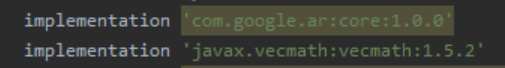
\includegraphics[width=0.9\textwidth]{Capture7.png}
	\newline
	\par
	Et nous avons spécifier les autorisation nécessaire pour la caméra et pour la connection internet qui nous servira par la suite.
	\newline
	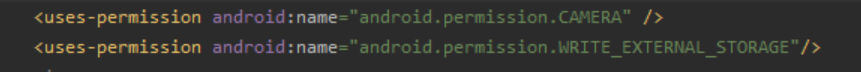
\includegraphics[width=0.9\textwidth]{Capture6.png}
	\newline
	\subsection{Deuxième partie}
	\par
	Après avoir réalisée la base de notre application de dessin nous avons commencé a réalisé la partie multi utilisateur. Cette partie sera réalisé en utilisant l'outil Firebase et le service RealTime Database.

	\par
	Nous avons tout d'abord créer un nouveau projet sur la page de FireBase afin de pouvoir ajouter le projet à notre application. A ce niveau il est nécessaire de renseigner le nom du package.
	\newline
	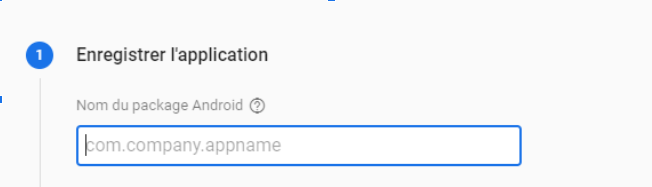
\includegraphics[width=0.9\textwidth]{Capture5.png}
	\newline
	\par
	Une fois cela réalisé Firebase donne un fichier .json à mettre dans notre application qui servira à se connecter au service. Il est nécessaire ici aussi de modifier le build du projet pour installer le service Firebase
	\newline
	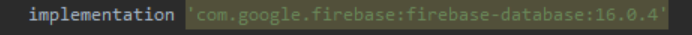
\includegraphics[width=0.9\textwidth]{Capture4.png}
	\newline
	\par
	Une fois que tout est configurer et installer nous pouvons échanger avec notre base de donnée pour sauvegarder ,récupère ou modifier nos données.\newline
	Pour la structure nous avions choisit dans un premier temps une structure assez simple:
	\newline
	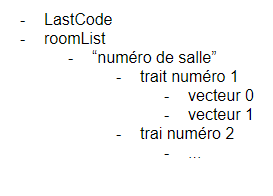
\includegraphics[width=0.35\textwidth]{Capture2.png}
	\newline
	\par
	Nous avions donc une variable nous rappelant la dernière pièce créer pour incrémenter cette dernière puis la liste des groupes où chaque groupe représenté la liste de vecteur.
	\par
	Mais ceci nous a posé problème car lorsqu'un joueur perdez la connexion ou que deux joueurs écrivaient en même temps, une des sauvegarde se trouve écrasée par la dernière envoyé. Nous avons donc changer la structure pour attribuer à chaque nouvelle utilisation du groupe, une liste personnelle que seul lui pouvait modifier sans toucher aux autres.
	\newline
	La nouvelle structure est donc :
	\newline
	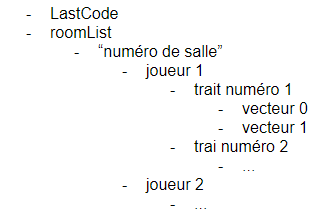
\includegraphics[width=0.5\textwidth]{Capture.png}
	\newline
\section{Validation et Application}
\par
Nous avons dans l'ensemble réalisé les fonctionnalités voulu dans notre application. Mais nous avons des fonctionnalité qui sont partiellement développé. L'application permet donc de créer un groupe d'utilisateur qui peuvent interagir sur l'environnement en dessinant.
\newline
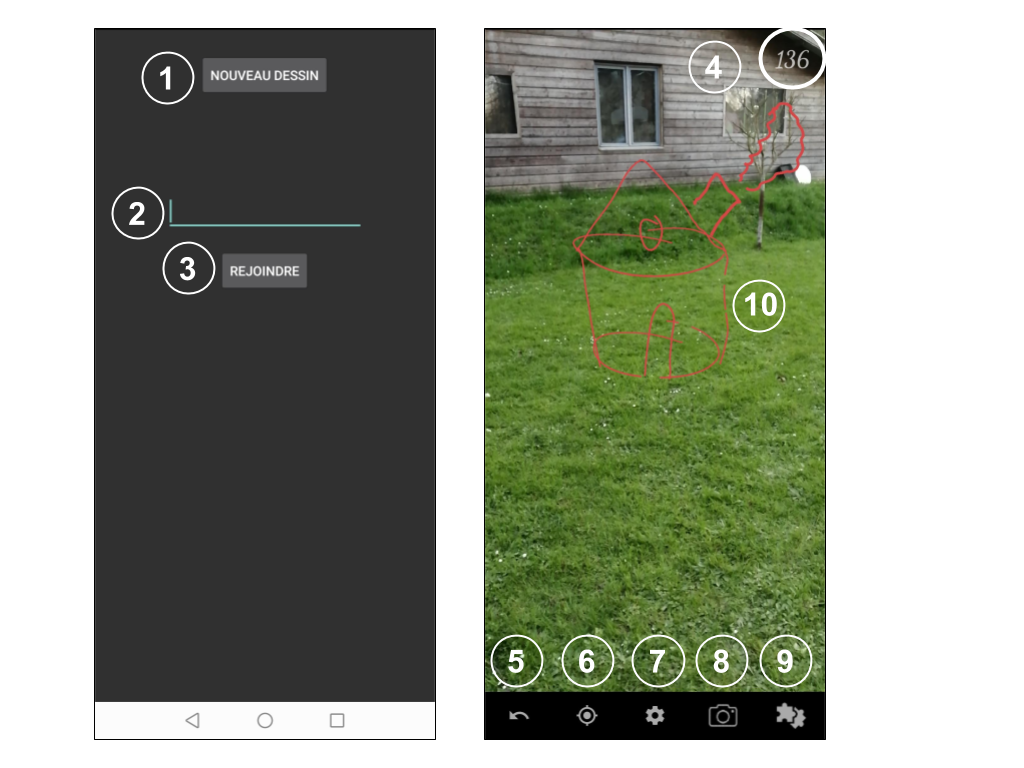
\includegraphics[width=1\textwidth]{dessin1.png}
\newline
\par
Lorsque l'utilisateur ouvre l'application deux choix luis son possible, Il peut créer un nouveau dessins \textbf{(1)} et un code lui sera attribué \textbf{(4)}. Ou si une session est déjà lancé et qu'il dispose du code il peut le rentrer \textbf{(2)} et se connecter au dessin \textbf{(3)}.
Une fois cette étape passée l'utilisateur peut commencer à dessiner \textbf{(10)} et verra les dessin des autre joueur s'ajouter au sien et vice versa .
Plusieurs boutons lui sont disponibles , il peut effacer le dernier trait réaliser \textbf{(5)} ,modifier la position du dessin en générale \textbf{(6)}, modifier la couleur des traits \textbf{(7)} valider le dessin \textbf{(8)} et afficher le modèle.

\begin{center}		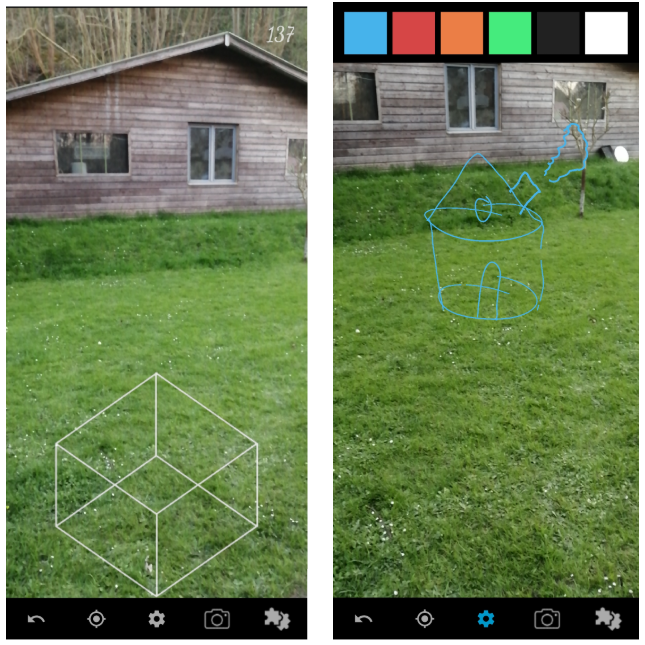
\includegraphics[width=0.65\textwidth]{Capture3.png}
\end{center}

\begin{center}		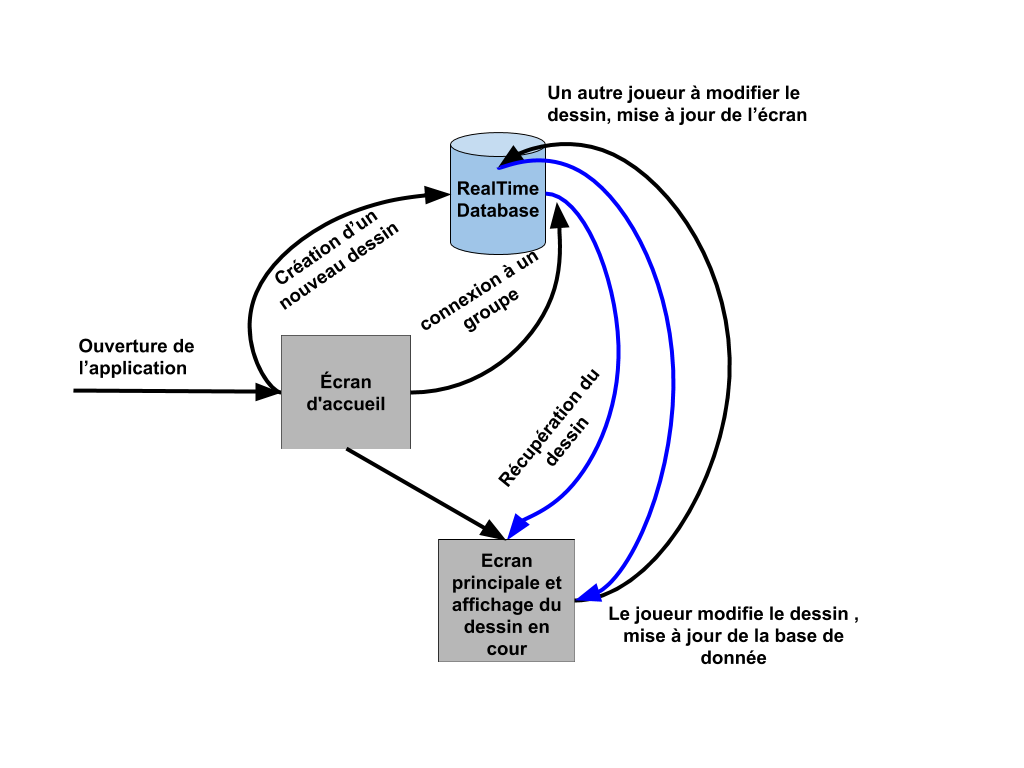
\includegraphics[width=0.85\textwidth]{dessin2.png}
\end{center}

\section{Conclusion}
Notre projet consistait à créer une application de réalité augmentée concrète. Le projet de l'année dernière était une bonna base sur laquelle s'appuyer mais nous avons décidé de créer un jeu n'utilisant pas les technologies utilisés lors de ce projet. Il nous fallut reprendre de zéro. Après avoir choisis d'utiliser  ARcore qui convenait le mieux à notre projet pour ses caractéristique et la base de données Firebase, nous avons mis en place le logiciel de dessin avec l'aide de DrawAR. Nous avons ensuite intégré le multi utilisateur en temps réel après plusieurs tests et essais qui nous permirent d'en apprendre plus sur cette technologie. Aujourd'hui, l'application peut toujours être améliorer dans le futur en créant l'algorithme de reconnaissance de dessin mais l'objectif de création de cette application multi utilisateur est un succès. Cependant, dû aux événements de ces derniers jours, l'objectif de la journée de validation posa des problèmes et nous ne pûmes pas réaliser cet objectif.
\newline
Ce projet fut pour nous extrêmement intéressant et original. Nous vous invitons à prendre connaissance de l'aspect pédagogique de ce projet dans le rapport pédagogique.
\section{Annexe}
\textbf{Différent liens lié à la création de notre projet:}
\newline
\newline
\textbf{Vous pouvez retrouver ici le lien vers le projet réalisé : }
\newline
\href{https://github.com/Deathpioupiou/Project_master_1}{\text{https://github.com/Deathpioupiou/Project$\_master\_1$}}
\newline
\newline
\textbf{Lien du projet DrawAR:}
\newline
\href{https://github.com/googlecreativelab/ar-drawing-java/blob/master/app/src/main/java/com/googlecreativelab/drawar/DrawAR.java}{\text{https://github.com/googlecreativelab/ar-drawing-java/blob/master/app/src/main/java/com/googlecreativelab/drawar/DrawAR.java}}
\newline
\newline
\textbf{Lien de la documentation d'ARcore : }
\newline
\href{https://developers.google.com/ar/reference/java}{\text{https://developers.google.com/ar/reference/java}}
\newline
\newline
\textbf{Lien de la documention FireBase : }
\newline
\href{https://firebase.google.com/docs/database}{\text{https://firebase.google.com/docs/database}}

\end{document}